\chapter{Assignment: Model Explanation}
\label{hw:model-explanation}

\newthought{Understanding the model is essential for decision-making.}\marginnote{For this assignment, we will be using Explain add-on, which you can install in Options -- Add-ons.} We will be using \textit{Attrition - Train} data from the \widget{Datasets} widget. We already know the data and its properties. But for reaching any kind of decisions regarding employee attrition, it is important not only to evaluate the models, but to understand them - what they do, which features are important, and in what way.

\begin{figure*}[h]
  \centering
  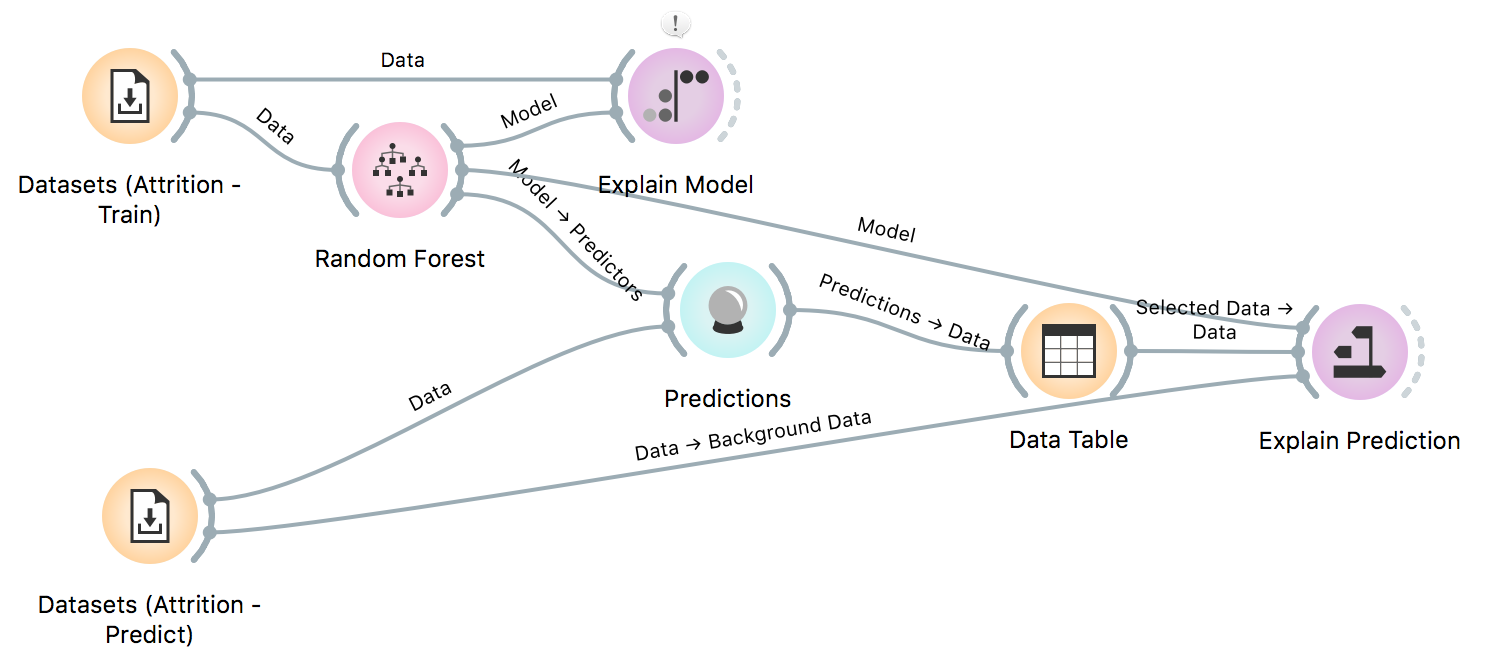
\includegraphics[width=\linewidth]{workflow.png}%
  \caption{$\;$}
\end{figure*}

Use \widget{Random Forest} to train a model, then answer the following questions:
\begin{enumerate}
    \item Looking at \widget{Explain Model}, which are the top three features for the random forest model?
    \item Change the target class to \textit{Yes}. What happens?
    \item Two of the top three features are the same. Why?
    \item In \widget{Data Table}, select the employee for whom you wish to explain the prediction. Say, we go with John. Will John likely stay with the company or resign? Look at \widget{Predictions} for an answer.
    \item In \widget{Explain Predictions}, explain \emph{why} John is leaving or staying.
\end{enumerate}
